\chapter{Analýza dekarbonizace výroby vodíku v rafinérii}

Praktická část této bakalářské práce je rozdělena na dvě části. V první části bude odhadnuta produkce \ce{CO2} na kilogram vyrobeného vodíku na jednotce parciální oxidace při zplyňování těžkých topných olejů. V druhé části bude provedeno naznačení částečné i úplné dekarbonizace modelové výroby vodíku v rafinérii, tedy nahrazení výroby šedého vodíku z jednotky parciální oxidace vodíkem pocházejícího z elektrolyzérů za využití elektrické energie pocházející z lokální solární elektrárny. Výpočet bude proveden na základně dat z výše zmiňované tuzemské rafinérie \textit{Orlen Unipetrol}.

\section{Model jednotky parciální oxidace těžkých topných olejů}

Vodík, který je převážně určen pro potřeby rafinérie, je vyráběn na jednotce parciální oxidace, jejíž fungování je popsáno v teoretické části práce. Pro správné určení reaktantů a produktů parciální oxidace těžkých topných olejů \acs{TTO} bude sestaven zjednodušený model parciální oxidace kyslíkem a vodní parou s využitím rovnic (3.6) a (3.7). Bude uvažován souběžný průběh reakcí a poměr vstupujícího kyslíku a vody 1:1 mol. Zmíněné rovnice tedy lze sečíst a a zjednodušit na tvar
\reaction{\mathrm{C_mH_n} + \frac{1}{2} mO2 + \frac{1}{2} mH2O -> \frac{1}{2} mCO2 + \frac{1}{2} mCO + $\left(\mathrm{\frac{1}{2} m + \frac{1}{2} n}\right)$H2}
Dále je nutné předpokládat, že vzniklý oxid uhelnatý reaguje s kyslíkem a tvoří oxid uhličitý dle této reakce
\reaction{mCO + \frac{1}{2} mO2 -> mCO2}
Nyní lze tyto rovnice sečíst a výsledná rovnice pro parciální oxidaci bude mít tvar
\reaction{\mathrm{C_mH_n} + \frac{2}{3} mO2 + \frac{2}{3} mH2O -> mCO2 + $\left(\mathrm{\frac{2}{3} m + \frac{1}{2} n}\right)$H2}
Pro další výpočty je vhodné zavést koeficienty, které zjednoduší prezentaci výsledků. Rovnici lze tedy upravit například následovně
\reaction{\mathrm{C_mH_n} + \mathrm{x} O2 + \mathrm{x} H2O -> \mathrm{y} CO2 + \mathrm{z} H2}
kde koeficienty x,y a z jsou zavedeny takto
\begin{equation}
    \mathrm{x} = \frac{2}{3}\mathrm{m} \quad \wedge \quad \mathrm{y} = \mathrm{m} \quad \wedge \quad \mathrm{z} = \mathrm{\frac{2}{3} m + \frac{1}{2} n}
\end{equation}
\label{eq:koeficienty}

Do jednotky parciální oxidace vstupuje těžký topný olej, jehož přesné složení není známo. Jedná se o těžký uhlovodíky nízké kvality, jejichž délka řetězce uhlíkových atomů může být v rozmezí $12 \div 70$. \cite{Beskoski2011} Pro zjednodušení následujících výpočtu byl těžký topný olej reprezentován variantně jako \textit{oktadekan} \ce{C18H38} s teplotou varu $317\ \mathrm{^{\circ}C}$ \cite{Oktadekan} a \textit{heneikosan} \ce{C21H44} s teplotou varu $356\ \mathrm{^{\circ}C}$ \cite{Heneikosan}. Pro tyto náhrady \acs{TTO} lze vypočíst koeficienty x,y a z dle rovnic (\ref{eq:koeficienty}) takto
\begin{table}[h]
    \centering
    \begin{tabular}{|c|c|c||c|c|c|}
        \hline
        \textbf{Uhlovodík} & Koef. \textbf{m} & Koef. \textbf{n} & Koef. \textbf{x} & Koef. \textbf{y} & Koef. \textbf{z}\\ \hline\hline
        oktadekan \ce{C18H38} & 18 & 38 & 12 & 18 & 31 \\ \hline
        heneisokan \ce{C21H44} & 21 & 44 & 14 & 21 & 36\\ \hline
    \end{tabular}
    \caption[Koeficienty uhlovodíků]{Koeficienty uhlovodíků}
    \label{tab:koeficienty}
\end{table}

V následujících podkapitolách bude za využití znalosti reakce (5.3), resp. (5.4) vypočteno, kolik bude vyprodukováno oxidu uhličitého vztaženo na jeden kilogram vyrobeného vodíku metodou parciální oxidace \acs{TTO}.

\subsection{Uvažování oktadekanu jako modelu suroviny}
\label{subsec:oktadekan}

Pro uhlovodík \ce{C18H38}, systematickým názvem \enquote{oktadekan}, platí dle Tab. \ref{tab:koeficienty} následující rovnice rozkladu
\reaction{C18H38 + 12O2 + 12H2O -> 18CO2 + 31H2}

Zvyklostí nejen v rafinérském průmyslu bývá uvádět množství produktu v jednotkách hmotnosti, tedy kilogramech a jeho násobcích. Bude tedy proveden přepočet z látkového množství na kilogramy, za znalosti následujícího vztahu
\begin{equation}
    M = \frac{m}{n} \Rightarrow m = M \cdot n \quad\quad \mathrm{[kg] = [kg\krat kmol^{-1}]\krat[kmol]}
\end{equation}
\label{eq:mol}
Pro výpočet esenciální molární hmotnosti $M$ látek jsou běžně dostupné v chemických tabulkách. Výčet potřebných pro následující výpočty je uveden v Tab. \ref{tab:molarni_hmotnosti}
\begin{table}[h]
    \centering
    \begin{tabular}{|c|c|c|}
        \hline
        \textbf{Látka} & Molární hmotnost $M\ [\mathrm{kg\krat kmol^{-1}}]$ & Zdroj \\ \hline\hline
        oktadekan \ce{C18H38} & $254,494$ & \cite{Oktadekan}\\ \hline
        heneisokan \ce{C21H44} & $296,574$ & \cite{Heneikosan}\\ \hline
        kyslík \ce{O2} & $32$ & \cite{Oxygen_M}\\ \hline
        voda \ce{H2O} & $18$ & \cite{Water_M}\\ \hline
        oxid uhličitý \ce{CO2} & $44$ & \cite{CD_M}\\ \hline
        vodík \ce{H2} & $2$ & \cite{Hydrogen_M}\\ \hline
    \end{tabular}
    \caption[Molární hmotnosti všech reaktantů a produktů]{Molární hmotnosti všech reaktantů a produktů}
    \label{tab:molarni_hmotnosti}
\end{table}

Rovnici (5.6) lze s využitím molárních hmotností v Tab. \ref{tab:molarni_hmotnosti} a vztahu \ref{eq:mol} přepsat takto: 
\reaction{$254,494$\ \mathrm{kg} \ C18H38 + $384$\ \mathrm{kg}\ O2 + $216$\ \mathrm{kg}\ H2O -> $792$\ \mathrm{kg}\ CO2 + $62$\ \mathrm{kg}\ H2}
Úpravou této rovnice lze zjistit, že z $1\ \mathrm{kg}$ oktadekanu, lze vyprodukovat $0,242\ \mathrm{kg}$ vodíku a $3,112\ \mathrm{kg}$ oxidu uhličitého. Nebo také na $1\ \mathrm{kg}$ vyrobeného vodíku připadá $12,75\ \mathrm{kg}$ vyprodukovaného oxidu uhličitého.

\subsection{Uvažování heneisokanu jako modelu suroviny}

V této podkapitole bude proveden stejný výpočet jako v předchozí podkapitole, se změnou pouze v použitém modelu suroviny v tomto případě tedy uhlovodíku \ce{C21H44} se systematickým názvem \enquote{heneisokan}. Rovnice rozkladu má tedy tvar
\reaction{C21H44 + 14O2 + 14H2O -> 21CO2 + 36H2}
v roznásobeném tvaru a přepočtu na kilogramy
\reaction{$296,574$\ \mathrm{kg} \ C18H38 + $448$\ \mathrm{kg}\ O2 + $252$\ \mathrm{kg}\ H2O -> $924$\ \mathrm{kg}\ CO2 + $72$\ \mathrm{kg}\ H2}
Z této rovnice vyplývá, že na $1\ \mathrm{kg}$ heneisokanu připadá vyrobených $0,243\ \mathrm{kg}$ vodíku a $3,19\ \mathrm{kg}$ oxidu uhličitého. Na $1\ \mathrm{kg}$ vyrobeného vodíku pak připadá $12,83\ \mathrm{kg}$ vyprodukovaného oxidu uhličitého.

\subsection{Vyhodnocení vlivu modelové suroviny pro výrobu vodíku parciální oxidací těžkých topných olejů}

Rozdíl mezi uvažováním oktadekanu a heneisokanu jako modelové suroviny pro parciální oxidaci je zanedbatelný. Hodnoty vyprodukovaného oxidu uhličitého na $1\ \mathrm{kg}$ vyrobeného vodíku se od sebe liší o $\approx 0,6\%$. Pro následující výpočty budou zvoleny výsledky oktadekanu. V následující kapitole budou tyto výsledky důležité pro stanovení velikosti znečištění životního prostředí vypuštěním oxidu uhličitého do ovzduší, při částečném, nebo úplném nahrazení výroby vodíku pomocí elektrolýzy.

\section{Nahrazení výroby vodíku elektrolýzou vody}

Litvínovská rafinérie má Ministerstvem životního prostředí České republiky dle IPPC způsobu regulace průmyslových činností stanovenou maximální dovolenou produkci vodíku zplyňováním mazutu, resp. \acs{TTO} $960\krat10^6\ \mathrm{Nm^3_{H_2}}/$rok. \cite{MZP2012} Při znalosti hustoty vodíku $0,089\ \mathrm{kg\krat Nm^{-3}}$ lze dopočíst dovolenou produkci vodíku v kilogramech. \cite{IEAreview}
\begin{equation}
    \rho = \frac{m}{V} \Rightarrow m = \rho \krat V = 0,089\krat960\krat10^6 = 85\ 440\ \mathrm{t}
\end{equation}
Ze zprávy o trvale udržitelném rozvoji skupiny \textit{Orlen Unipetrol} za rok 2022 \cite{unipetrol_zprava} vyplývá, že metodou parciální oxidace \acs{TTO} vyrobí v litvínovské rafinérii $80\ 000\ \mathrm{t}$ vodíku ročně. V následujících výpočtech bude proveden návrh částečné a úplné dekarbonizace litvínovské rafinérie pomocí \acs{PEM} elektrolyzérů, které by potenciálně nahradily produkci $80\ 000\ \mathrm{t}$ vodíku ročně z $5\%$, $10\%$, $15\%$ a $100\%$ roční produkce.

\subsection{Návrh elektrolyzérů}

Nejprve je nutné stanovit předpokládanou produkci obnovitelného vodíku při nahrazení z $5\%$, $10\%$, $15\%$ a $100\%$. Tato produkce je uvedená v Tab. \ref{tab:h2_rocni_produkce}, kde přepočet z $\mathrm{t_{H_2}}/$rok na $\mathrm{Nm^3_{H_2}}/$rok je určen dle definice hustoty látky takto
\begin{equation}
    V\ [\mathrm{Nm^3_{H_2}/rok}] = \frac{m\ [\mathrm{t_{H_2}/rok}]}{\rho}
\end{equation}

\newpage
\begin{table*}[h!]
    \centering
    \begin{tabular}{|c|c|c|}
        \hline
        Náhrada obnovitelným vodíkem & $5\%$ & $10\%$\\ \hline\hline
        Předpokládaná prod. [$\mathrm{t_{H_2}}/$rok] & $4\ 000$ & $8\ 000$\\ \hline
        Předpokládaná prod. [$\mathrm{Nm^3_{H_2}}/$rok] & $44\ 469\ 914$ & $88\ 939\ 828$\\ \hline
    \end{tabular}
\end{table*}
\begin{table}[h!]
    \centering
    \begin{tabular}{|c|c|c|}
        \hline
        Náhrada obnovitelným vodíkem & $15\%$ & $100\%$\\ \hline\hline
        Předpokládaná prod. [$\mathrm{t_{H_2}}/$rok] & $12\ 000$ & $80\ 000$\\ \hline
        Předpokládaná prod. [$\mathrm{Nm^3_{H_2}}/$rok] & $133\ 409\ 742$ & $889\ 398\ 281$\\ \hline
    \end{tabular}
    \caption[Roční produkce zeleného vodíku]{Roční produkce zeleného vodíku}
    \label{tab:h2_rocni_produkce}
\end{table}
\noindent
Při uvažování předběžného počtu $8000$ provozních hodin elektrolyzéru v roce lze zjistit předpokládanou produkci vodíku vztaženou na $1$ provozní hodinu.
\begin{table}[h]
    \centering
    \begin{tabular}{|c|c|c|c|c|}
        \hline
        Náhrada obnovitelným vodíkem & $5\%$ & $10\%$ & $15\%$ & $100\%$\\ \hline\hline
        Předpokládaná prod. [$\mathrm{t_{H_2}}/$h] & $500$ & $1\ 000$ & $1\ 500$ & $10\ 000$\\ \hline
        Předpokládaná prod. [$\mathrm{Nm^3_{H_2}}/$h] & $5559$ & $11\ 117$ & $16\ 676$ & $111\ 175$\\ \hline
    \end{tabular}
    \caption[Hodinová produkce vodíku zeleného vodíku]{Hodinová produkce vodíku zeleného vodíku}
    \label{tab:h2_hodinova_produkce}
\end{table}

\noindent
Na tyto hodnoty byly dimenzovány velikost a počet elektrolyzérů. Elektrolyzéry byly vybrány z řady \enquote{M} PEM elektrolyzérů společnosti \textit{Nel ASA} \cite{prakticka_elektrolyzer}.
\begin{table}[h!]
    \centering
    \begin{tabular}{|c|c|c|c|c|}
        \hline
        Náhrada obnovitelným vodíkem & $5\%$ & $10\%$ & $15\%$ & $100\%$\\ \hline
        Předpokládaná prod. [$\mathrm{Nm^3_{H_2}}/$h] & $5\ 559$ & $11\ 117$ & $16\ 676$ & $111\ 175$\\ \hline\hline
        2x PEM elektrolyzér M3000 [$\mathrm{Nm^3_{H_2}}/$h] & $5\ 904$ & & & \\ \hline
        3x PEM elektrolyzér M4000 [$\mathrm{Nm^3_{H_2}}/$h] & & $11\ 808$ & & \\ \hline
        6x PEM elektrolyzér M3000 [$\mathrm{Nm^3_{H_2}}/$h] & & & $17\ 712$ & \\ \hline
        23x PEM elektrolyzér M5000 [$\mathrm{Nm^3_{H_2}}/$h] & & & & $113\ 160$ \\ \hline
    \end{tabular}
    \caption[Předpokládaná a nominální a hodinová produkce vodíku vybraných elektrolyzérů]{Předpokládaná a nominální a hodinová produkce vodíku vybraných elektrolyzérů}
    \label{tab:vybrane_elektrolyzery}
\end{table}

\noindent
Po zvolení elektrolyzérů je nutné aktualizovat počet provozních hodin pro instalovanou kapacitu elektrolyzérů na reálnou hodnotu, která se stanoví podílem předpokládané roční produkce vodíku a výrobní kapacity jednotky elektrolyzérů.
\begin{table*}[h!]
    \centering
    \begin{tabular}{|c|c|c|}
        \hline
        Náhrada obnovitelným vodíkem & $5\%$ & $10\%$\\ \hline
        Předpokládaná prod. [$\mathrm{Nm^3_{H_2}}/$rok] & $44\ 469\ 914$ & $88\ 939\ 828$\\ \hline
        Výrobní kap. elektrolyzérů [$\mathrm{Nm^3_{H_2}}/$h] & $5\ 904$ & $11\ 808$\\ \hline\hline
        Provozní hodiny instalované kap.& $7\ 532$ & $7\ 532$\\ \hline
    \end{tabular}
\end{table*}
\begin{table}[h!]
    \centering
    \begin{tabular}{|c|c|c|}
        \hline
        Náhrada obnovitelným vodíkem & $15\%$ & $100\%$\\ \hline
        Předpokládaná prod. [$\mathrm{Nm^3_{H_2}}/$rok] & $133\ 409\ 742$ & $889\ 398\ 281$\\ \hline
        Výrobní kap. elektrolyzérů [$\mathrm{Nm^3_{H_2}}/$h] & $17\ 712$ & $113\ 160$ \\ \hline\hline
        Provozní hodiny instalované kap.& $7\ 532$ & $7\ 860$ \\ \hline
    \end{tabular}
    \caption[Stanovení počtu provozních hodin instalované kapacity]{Stanovení počtu provozních hodin instalované kapacity}
    \label{tab:provozni_hodiny}
\end{table}

\newpage
\noindent
Z katalogového listu vybraných elektrolyzérů lze zjistit, že průměrná spotřeba elektrické energie na vystavěnou jednotky je $4,5\ \mathrm{kWh/Nm^3_{H_2}}$. Ze spotřeby a výrobní kapacity elektrolyzérů lze vypočítat výkon jednotlivých elektrolyzérů, potažmo celé jednotky v $\mathrm{MW}$. Hodnoty pro všechny jednotky jsou uvedené v Tab. \ref{tab:vykony}.
\begin{table}[h]
    \centering
    \begin{tabular}{|c|c|c|c|c|}
        \hline
        Náhrada obnovitelným vodíkem & $5\%$ & $10\%$ & $15\%$ & $100\%$\\ \hline
        Výrobní kap. elektrolyzérů [$\mathrm{Nm^3_{H_2}}/$h] & $5\ 904$ & $11\ 808$ & $17\ 712$ & $113\ 160$ \\ \hline
        Spotřeba el. energie jednotky [$\mathrm{kWh/Nm^3_{H_2}}$] & $4,5$ & $4,5$ & $4,5$ & $4,5$ \\ \hline\hline
        Výkon jednotky elektrolyzérů [$\mathrm{MW}$] & $27$ & $54$ & $80$ & $510$ \\ \hline
    \end{tabular}
    \caption[Stanovení výkonu elektrolyzérů]{Stanovení výkonu elektrolyzérů}
    \label{tab:vykony}
\end{table}

\subsection{Celkové provozní náklady chodu elektrolyzérů}

Do provozních nákladů jednotek PEM elektrolyzérů byly započteny pouze spotřebovaná elektrická energie a demineralizovaná voda, potřebná na uskutečnění reakce. Odpisy nebyly uvažovány. Celkovou spotřebu elektrické energie elektrolyzérů za rok lze vypočíst dle vztahu
\begin{align}
    \begin{split}
        \mathrm{\text{roční spotřeba el. energie}} =& \frac{\mathrm{produkce\ H_2} \cdot \mathrm{\text{průměrná spotřeba jednotky}}}{1000} \\
        [\mathrm{MWh/rok}] =& \frac{[\mathrm{Nm^3_{H_2}/rok}]\cdot[\mathrm{kWh/Nm^3_{H_2}}]}{1000}
    \end{split}
\end{align}

\noindent
Spotřebu demineralizované vody lze určit z předpokládané roční produkce vodíku, za znalosti měrné spotřeby demineralizované vody, která činí $10\ \mathrm{l/kg_{H_2}}$. \cite{SiemensEnergy2020} Hodnoty spotřeb elektrické energie a demineralizované vody jsou uvedeny v Tab. \ref{tab:spotreby}.
\begin{table*}[h!]
    \centering
    \begin{tabular}{|c|c|c|}
        \hline
        Náhrada obnovitelným vodíkem & $5\%$ & $10\%$\\ \hline
        Předpokládaná prod. [$\mathrm{t_{H_2}}/$rok] & $4\ 000$ & $8\ 000$\\ \hline
        Předpokládaná prod. [$\mathrm{Nm^3_{H_2}}/$rok] & $44\ 469\ 914$ & $88\ 939\ 828$\\ \hline\hline
        Spotřeba el. energie jednotky [$\mathrm{kWh/Nm^3_{H_2}}$] & $4,5$ & $4,5$\\ \hline\hline
        Měrná spotřeba demin. vody [$\mathrm{l/kg_{H_2}}$] & $10$ & $10$\\ \hline\hline
        Roční spotřeba el. energie [$\mathrm{MWh/rok}$] & $200\ 115$ & $400\ 229$ \\ \hline
        Roční spotřeba demin. vody [$\mathrm{l/rok}$] & $40\ 000\ 000$ & $80\ 000\ 000$\\ \hline
    \end{tabular}
\end{table*}
\begin{table}[h!]
    \centering
    \begin{tabular}{|c|c|c|}
        \hline
        Náhrada obnovitelným vodíkem & $15\%$ & $100\%$\\ \hline
        Předpokládaná prod. [$\mathrm{t_{H_2}}/$rok] & $12\ 000$ & $80\ 000$\\ \hline
        Předpokládaná prod. [$\mathrm{Nm^3_{H_2}}/$rok] & $133\ 409\ 742$ & $889\ 398\ 281$\\ \hline\hline
        Spotřeba el. energie jednotky [$\mathrm{kWh/Nm^3_{H_2}}$] & $4,5$ & $4,5$ \\ \hline\hline
        Měrná spotřeba demin. vody [$\mathrm{l/kg_{H_2}}$]& $10$ & $10$ \\ \hline\hline
        Roční spotřeba el. energie [$\mathrm{MWh/rok}$] & $600\ 334$ & $4\ 002\ 292$ \\ \hline
        Roční spotřeba demin. vody [$\mathrm{l/rok}$] & $120\ 000\ 000$ & $800\ 000\ 000$ \\ \hline
    \end{tabular}
    \caption[Spotřeba elektrické energie a demineralizované vody elektrolyzérů]{Spotřeba elektrické energie a demineralizované vody elektrolyzérů}
    \label{tab:spotreby}
\end{table}

Bude uvažována průměrná denní cena elektřiny v roce 2024 v ČR $2\ 265\ \mathrm{\text{Kč/MWh}}$ \cite{cena_elektriny} a cena demineralizované vody při odběru $10\ 000\ \mathrm{l}$ $2,5\ \mathrm{\text{Kč/l}}$ bez DPH \cite{cena_demivoda}. Za znalosti hodnot z Tab. \ref{tab:spotreby} lze vypočítat částku za spotřebovanou elektrickou energii a demineralizovanou vodu, které v součtu dají celkové provozní náklady chodu elektrolyzéru. Tyto náklady jsou vypočteny a uvedeny v Tab \ref{tab:naklady}.
\begin{table*}[h]
    \centering
    \begin{tabular}{|c|c|c|}
        \hline
        Náhrada obnovitelným vodíkem & $5\%$ & $10\%$\\ \hline
        Částka za elektrickou energii [Kč/rok] & $453\ 259\ 599$ & $906\ 519\ 198$ \\ \hline
        Částka za demin. vodu [Kč/rok] & $100\ 000\ 000$ & $200\ 000\ 000$ \\ \hline\hline
        Celkové provozní náklady [Kč/rok] & $553\ 259\ 599$ & $1\ 106\ 519\ 198$\\ \hline
    \end{tabular}
\end{table*}
\begin{table}[h]
    \centering
    \begin{tabular}{|c|c|c|}
        \hline
        Náhrada obnovitelným vodíkem & $15\%$ & $100\%$\\ \hline
        Částka za elektrickou energii [Kč/rok] & $1\ 359\ 778\ 797$ & $9\ 065\ 191\ 977$\\ \hline
        Částka za demin. vodu [Kč/rok] & $300\ 000\ 000$ & $2\ 000\ 000\ 000$\\ \hline\hline
        Celkové provozní náklady [Kč/rok] & $1\ 659\ 778\ 797$ & $11\ 065\ 191\ 977$\\ \hline
    \end{tabular}
    \caption[Spotřeba elektrické energie a demineralizované vody elektrolyzérů]{Spotřeba elektrické energie a demineralizované vody elektrolyzérů}
    \label{tab:naklady}
\end{table}

\subsection{Náklady na snížení emisí oxidu uhličitého}

Aby bylo možné zjistit potenciální náklady na snížení vypouštěného oxidu uhličitého při náhradě šedého vodíku zeleným vodíkem, je nutné od celkových provozních nákladů odečíst tržní cenu šedého vodíku vyprodukovaného parciální oxidací \acs{TTO}. Dle Obr. \ref{fig:cenyH2} bude zvolena cena šedého vodíku $2\ \mathrm{USD/kg_{H_2}}$, po přepočtu $47\ \mathrm{\text{Kč}/kg_{H_2}}$ \cite{usdtoczk}. Touto cenou bude vynásobena předpokládaná roční produkce zeleného vodíku a výsledná částka bude odečtena od celkových provozních nákladů.
\begin{table*}[h]
    \centering
    \begin{tabular}{|c|c|c|}
        \hline
        Náhrada obnovitelným vodíkem & $5\%$ & $10\%$\\ \hline
        Předpokládaná prod. [$\mathrm{t_{H_2}}/$rok] & $4\ 000$ & $8\ 000$\\ \hline\hline
        Celkové provozní náklady [Kč/rok] & $553\ 259\ 599$ & $1\ 106\ 519\ 198$\\ \hline
        Cena vyprodukovaného vodíku [Kč/rok] & $188\ 000\ 000$ & $376\ 000\ 000$\\ \hline\hline
        Náklady na snížení emisí \ce{CO2} [Kč/rok] & $365\ 259\ 599$ & $73\ 0519\ 198$\\ \hline
        \end{tabular}
\end{table*}
\begin{table}[h!]
    \centering
    \begin{tabular}{|c|c|c|}
        \hline
        Náhrada obnovitelným vodíkem &$15\%$ & $100\%$\\ \hline
        Předpokládaná prod. [$\mathrm{t_{H_2}}/$rok] & $12\ 000$ & $80\ 000$\\ \hline\hline
        Celkové provozní náklady [Kč/rok] & $1\ 659\ 778\ 797$ & $11\ 065\ 191\ 977$\\ \hline
        Cena vyprodukovaného vodíku [Kč/rok] & $564\ 000\ 000$ & $3\ 760\ 000\ 000$\\ \hline\hline
        Náklady na snížení emisí \ce{CO2} [Kč/rok] & $1\ 095\ 778\ 797$ & $7\ 305\ 191\ 977$\\ \hline
        \end{tabular}
    \caption[Náklady na snížení emisí \ce{CO2}]{Náklady na snížení emisí \ce{CO2}}
    \label{tab:nakladyco2}
\end{table}

\noindent
Z hodnoty vyprodukovaného oxidu uhličitého $12,75\ \mathrm{kg_{CO_2}/\mathrm{kg_{H_2}}}$, která byla odhadnuta v podkapitole \ref{subsec:oktadekan} pro výrobu vodíku pomocí parciální oxidace, lze určit absolutní úsporu potenciálně vyprodukovaného oxidu uhličitého vynásobením této hodnoty předpokládanou roční produkcí vodíku. Výpočet je proveden v Tab. \ref{tab:usporaco2}.
\newpage
\begin{table}[h!]
    \centering
    \begin{tabular}{|c|c|c|c|c|}
        \hline
        Náhrada obnovitelným vodíkem & $5\%$ & $10\%$ & $15\%$ & $100\%$\\ \hline
        Předpokládaná prod. [$\mathrm{t_{H_2}}/$rok] & $4\ 000$ & $8\ 000$ & $12\ 000$ & $80\ 000$\\ \hline\hline
        Uspořené \ce{CO2} [$\mathrm{t_{CO_2}}/$rok] & $51\ 000$ & $102\ 000$ & $153\ 000$ & $1\ 020\ 000$ \\ \hline
    \end{tabular}
    \caption[Úspora potenciálně vyprodukovaného oxidu uhličitého]{Úspora potenciálně vyprodukovaného oxidu uhličitého}
    \label{tab:usporaco2}
\end{table}

Měrné náklady na snížení emisí oxidu uhličitého se vypočítají se podle následujícího vztahu a dle definice by měly být stejné pro všechny případy, tedy $5\%$, $10\%$, $15\%$ a $100\%$ nahrazení produkce šedého vodíku zeleným vodíkem.
\begin{align}
    \begin{split}
        \text{náklady na ušetření} =& \frac{\text{náklady na snížení emisí}}{\text{uspořený oxid uhličitý}} \\
        [\text{Kč}/\mathrm{t_{CO_2}}] =& \frac{[\text{Kč/rok]}}{[\mathrm{t_{CO_2}/rok}]}
    \end{split}
\end{align}
Po dosazení např. pro variantu $5\%$ nahrazení produkce zeleným vodíkem (data viz. Tab. \ref{tab:nakladyco2} a Tab. \ref{tab:usporaco2}) tedy
\begin{equation}
    \text{náklady na ušetření} = \frac{365\ 259\ 599}{51\ 000} = 7\ 162\ \text{Kč}/\mathrm{t_{CO_2}}
\end{equation}

\subsection{Vyhodnocení dekarbonizace rafinérie}
Částečná nebo úplná dekarbonizace rafinérie se společnostem při aktuální ceně energie nevyplatí. Při průměrné ceně emisní povolenky\footnote{Obchodování s emisními povolenkami v Evropské unii slouží jako nástroj k redukci emisí skleníkových plynů v Evropě. \cite{emisni_povolenka}} v roce 2024 $1\ 678\ \mathrm{\text{Kč}/t_{\text{emisí}\mathrm{CO_2}}}$ jsou náklady na odstranění oxidu uhličitého až $4,1$krát vyšší, než odhadnuté náklady které z rovnice (5.16) činí $7\ 162\ \mathrm{\text{Kč}/t_{\text{emisí}\mathrm{CO_2}}}$. Do nákladů navíc nebyly započítané prvotní investiční náklady na nákup elektrolyzérů a vybudování vodíkové infrastruktury.

Náklady na snížení emisí oxidu uhličitého rostou lineárně s procentuální náhradou produkce zeleným vodíkem až do $100\%$. Náklady mohou být optimalizovány při výstavbě lokální solární, nebo větrné elektrárny, která by vyráběla elektrickou energii s nižšími náklady. Názorný výpočet a odhad potřebné plochy lokální solární elektrárny, která by mohla být v blízkosti litvínovské rafinérie je proveden v následující podkapitole.

\newpage
\subsection{Dimenzování solární elektrárny}

Lokalita uvažovaná pro výstavbu solární elektrárny v Litvínově-Záluží je v blízkosti tamní rafinérie, viz. Obr. \ref{fig:letecky_snimek}. Dle dat z katastru nemovitostí je areál ve vlastnictví společnosti \textit{Orlen Unipetrol} a má výměru $1\ 641\ 367\ \mathrm{m^2}$. \cite{katastr}
\begin{figure}[h!]
    \centering
    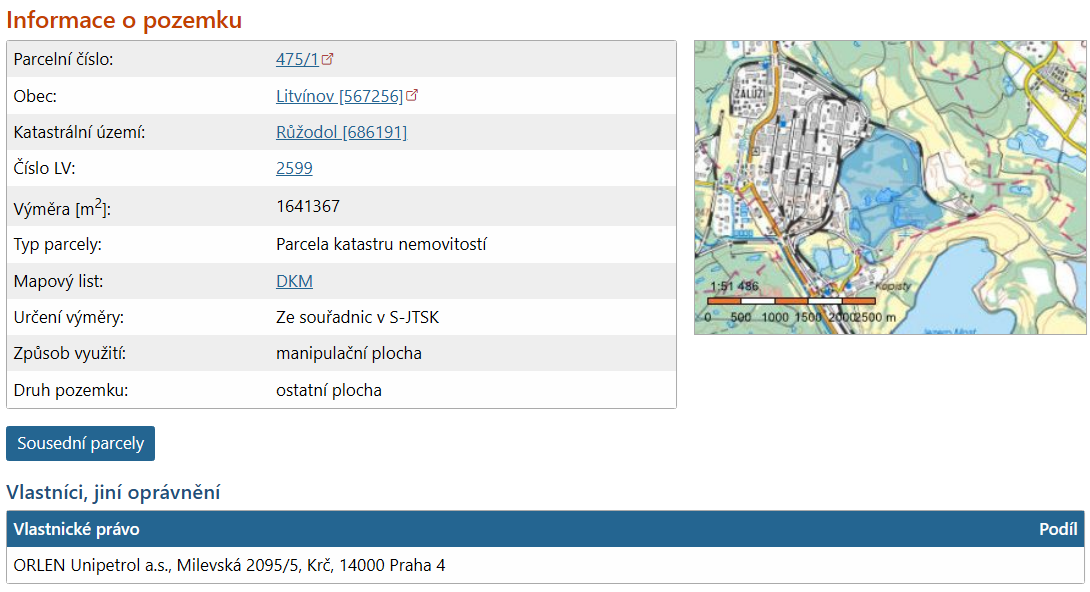
\includegraphics[width=.95\textwidth]{figures/katastr.png}
    \caption[Informace o pozemku pro potenciální výstavbu solární elektrárny]{Informace o pozemku pro potenciální výstavbu solární elektrárny \cite{katastr}.} \label{fig:katastr}
\end{figure}

\noindent
Bude-li uvažováno, že celá vyměřená plocha bude využita na výstavbu solární elektrárny, lze pomocí údajů o slunečním svitu dopadajícím na tuto lokalitu zjistit potenciální výkon solární elektrárny. Data o slunečním svitu jsou volně dostupné ve Fotovoltaickém a geografickém informačním systému (\acs{PVGIS}), který spadá pod Evropskou komisi. \cite{EuropeanComission2024} Pro danou lokalitu \enquote{Růžodol} jsou v systému \acs{PVGIS} dostupná tato data o slunečním záření za rok 2020
\begin{figure}[h]
    \centering
    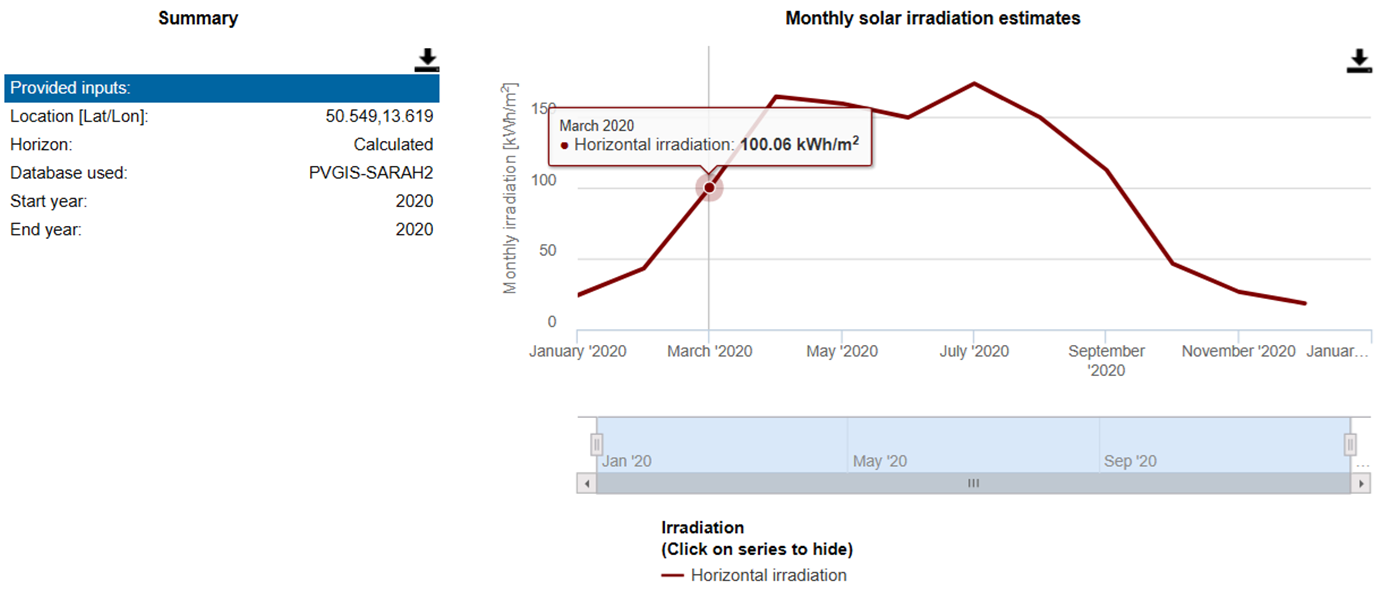
\includegraphics[width=.95\textwidth]{figures/zareni.png}
    \caption[Informace o slunečním zářením v lokalitě Růžodol]{Informace o slunečním zářením v lokalitě Růžodol \cite{EuropeanComission2024}.} \label{fig:zareni}
\end{figure}

\noindent
Na Obr. \ref{fig:zareni} jsou z grafu vybrána data za měsíc březen. Jedná se o odhadnutou průměrnou roční hodnotu, protože v létě bude přebytek vyrobené elektrické energie ze solárních panelů a naopak v zimě bude rafinérie čerpat ze sítě. Osvětlení za měsíc březen v roce $2020$ tedy potenciálně mohlo zajistit výrobu $100\ \mathrm{kWh}$ elektrické energie na $1\ \mathrm{m^2}$ osvětlené plochy. Dle následujícího vztahu lze za znalosti celkové plochy vypočítat, kolik by solární elektrárna vyrobila odhadem elektrické energie za rok.
\begin{align}
    \begin{split}
        E_{el.} =& \ \text{osvit} \cdot \text{plocha} = 100\cdot1\ 641\ 367 = 164\ 136\ 700\ \mathrm{kWh} = 164\ 138\ \mathrm{MWh}\\
        [\mathrm{kWh}] =& [\mathrm{kWh/m^2}] \cdot [\mathrm{m^2}]
    \end{split}
\end{align}

\subsection{Vyhodnocení důležitosti lokální solární elektrárny}

V Tab. \ref{tab:spotreby} jsou vypočteny roční spotřeby energie elektrolyzérů vyrábějící zelený vodík. Pokud by lokální solární elektrárna vyráběla $164\ 138\ \mathrm{MWh}$ elektrické energie ročně, pokryla by tuto spotřebu elektrické energie při nahrazení $5\%$ výroby obnovitelným vodíkem z $82\%$. Při ceně elektrické energie od dodavatelů je výstavba lokální solární elektrárny pro dekarbonizaci rafinérie, i přes vysoké počáteční náklady, významně důležitá. Příklad byl proveden pro solární elektrárnu, avšak obdobný postup by následoval i při nahrazení odebírané elektrické energie lokální větrnou elektrárnou, které jsou častěji využívané v přístavních městech, jako je v předchozí kapitole zmíněný nizozemský Rotterdam.